% !TeX root = document.tex
% !TeX encoding = UTF-8 Unicode

\chapter{Gráficos}%
\label{chapter:graficos}

Esse módulo exibe os gráficos dos testes realizados e do teste em execução. Nele
é possível visualizar os sinais em tempo real durante a execução do teste. Nos
testes finalizados é possível exportar os dados. Na Figura~\ref{fig:graphs1}
podemos ver a listagem de gráficos com as opções pertinentes. O botão
\textit{Parar} funciona como nos módulos \textit{Resposta do Sistema} e
\textit{Controle do Sistema}.

\begin{figure}[ht!]
    \centering
    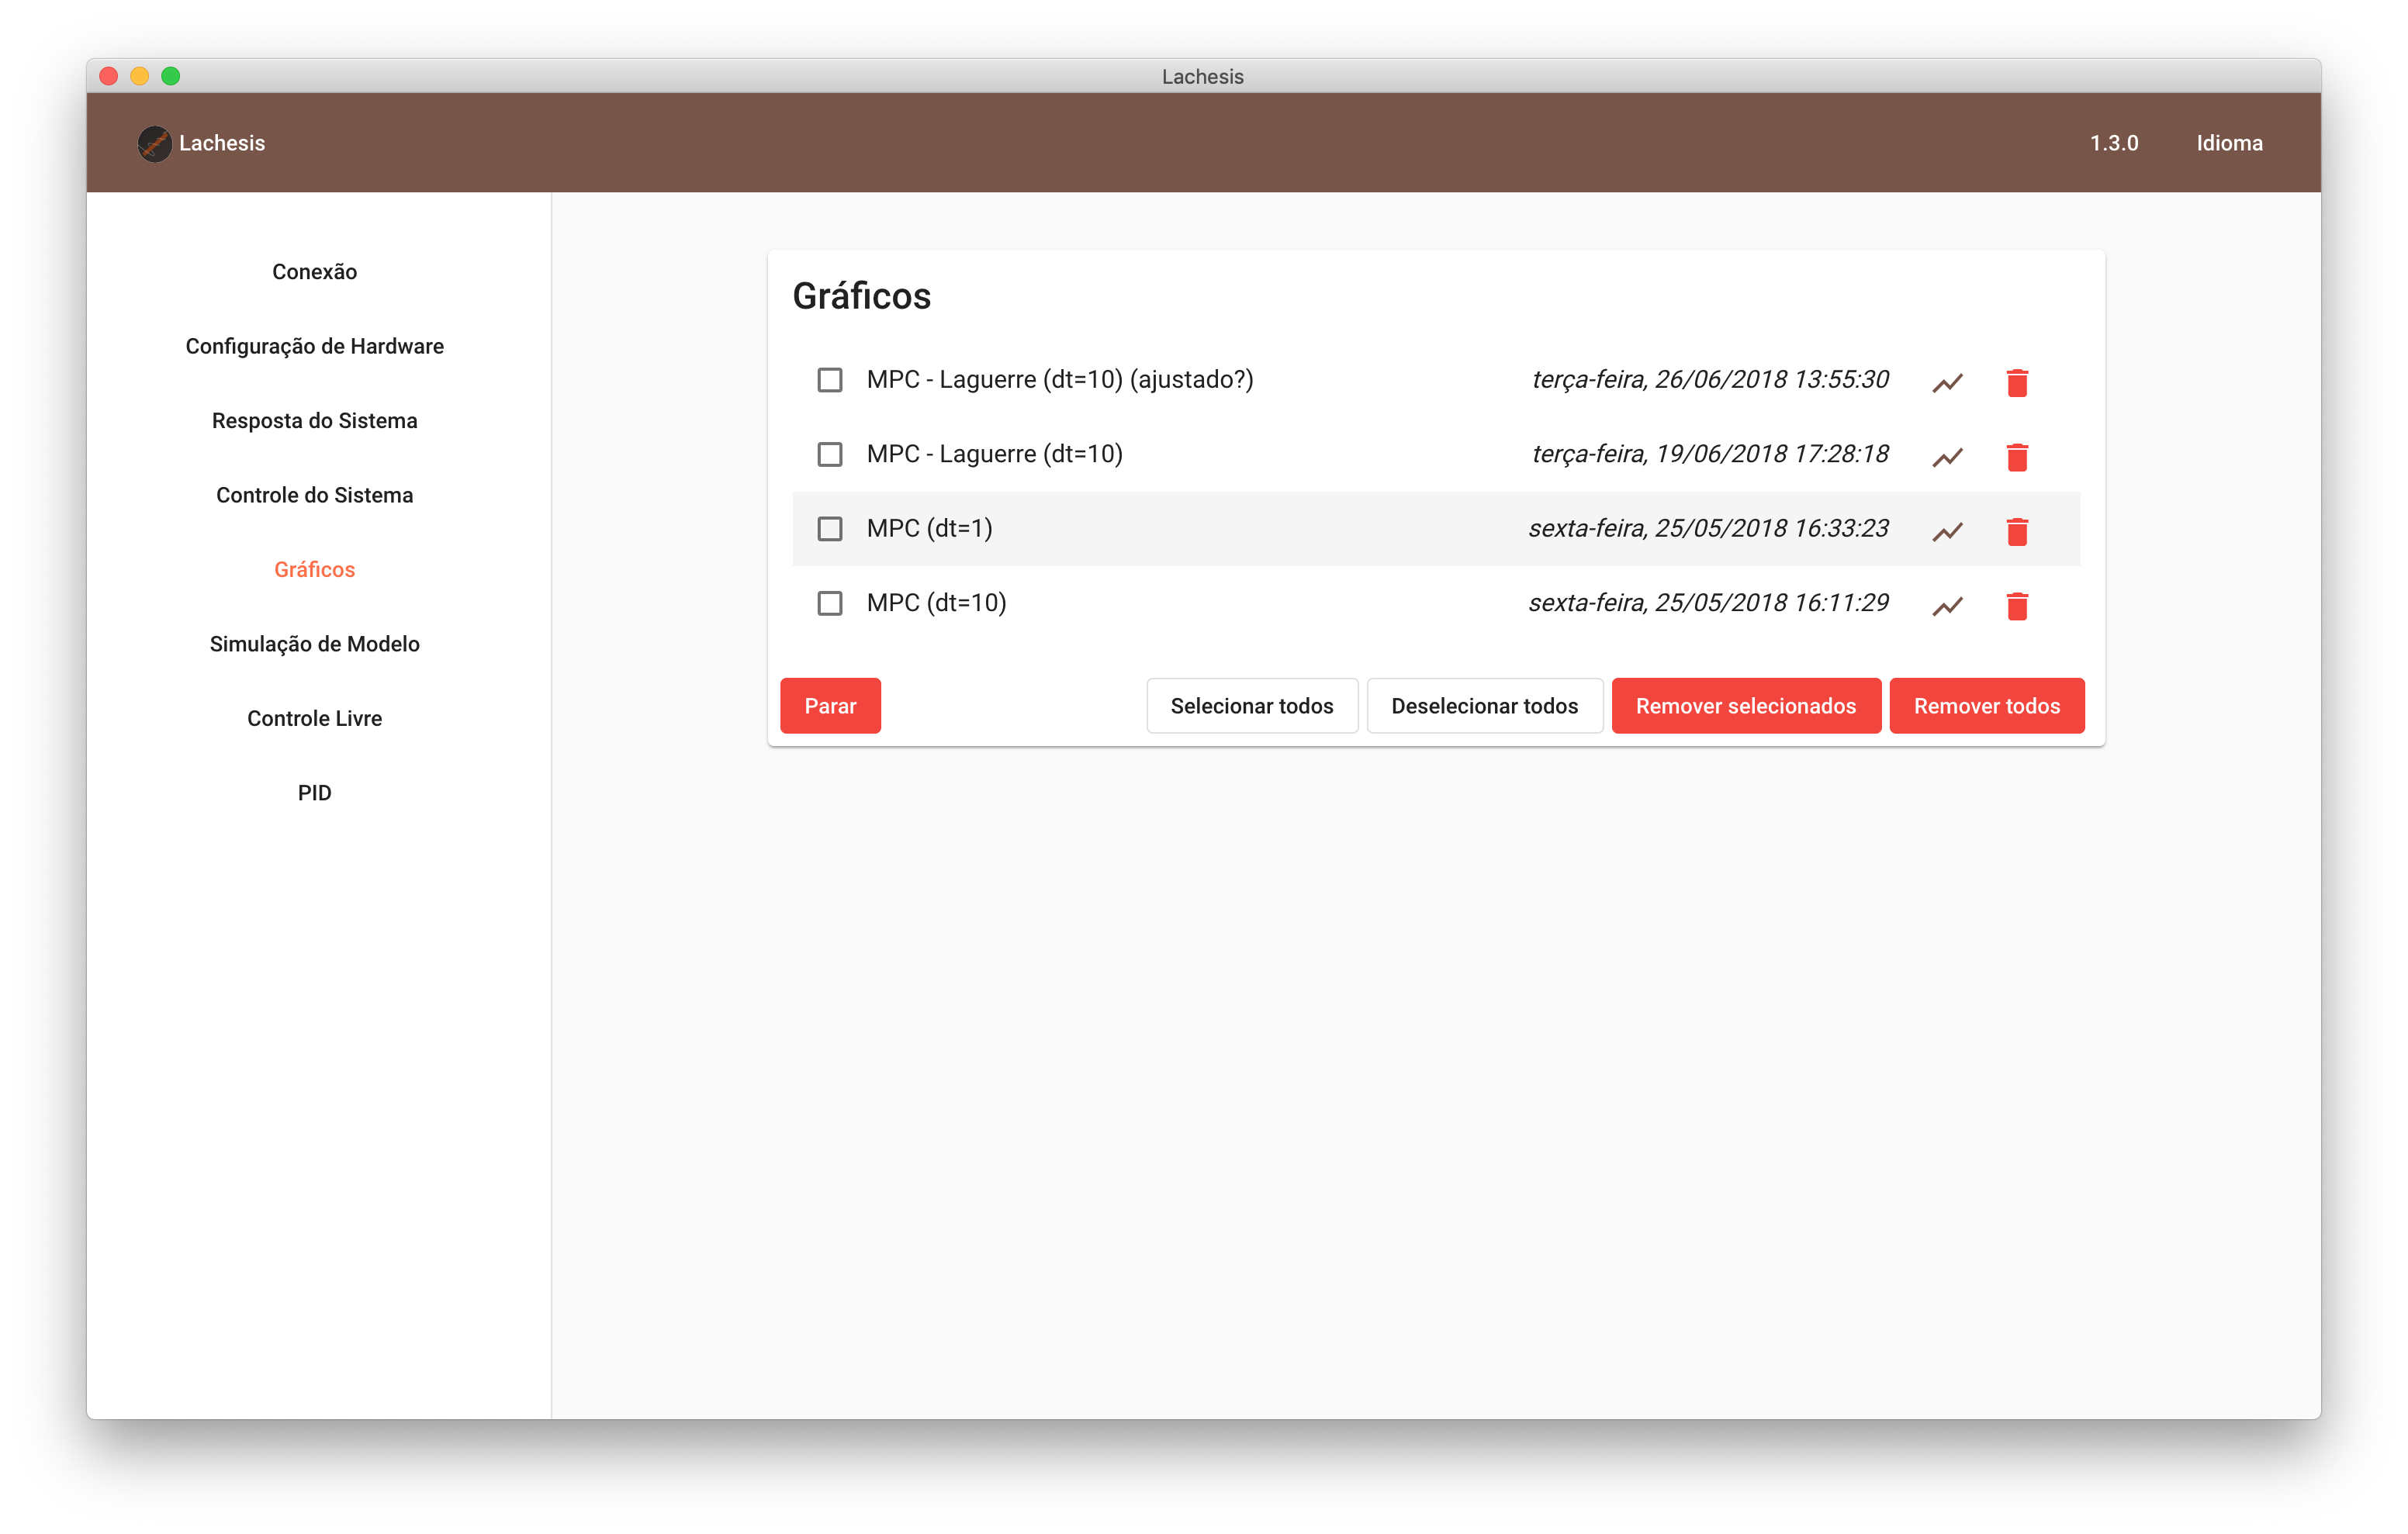
\includegraphics[width=0.9\textwidth]{imgs/graphs1}
    \caption[Módulo Gráficos]{Módulo Gráficos}%
    \label{fig:graphs1}
\end{figure}

Ao clicar em \textit{Exibir} (\img{imgs/show_chart}), a seção \textit{Gráficos}
será exibida. A seção \textit{Exportar} também aparecerá, mas apenas caso o
teste não esteja em execução. A seção \textit{Exportar} é retrátil, se
expandindo ao clicar no título ou botão no lado direito. Na
Figura~\ref{fig:graphs2} pode-se ver a seção expandida. No topo pode-se
selecionar o formato dos dados exportados: \href{https://www.json.org/}{JSON},
\href{https://pt.wikipedia.org/wiki/Comma-separated_values}{CSV} ou
\href{https://www.mathworks.com/help/matlab/import_export/supported-file-formats.html}{MAT}.

\begin{figure}[ht!]
    \centering
    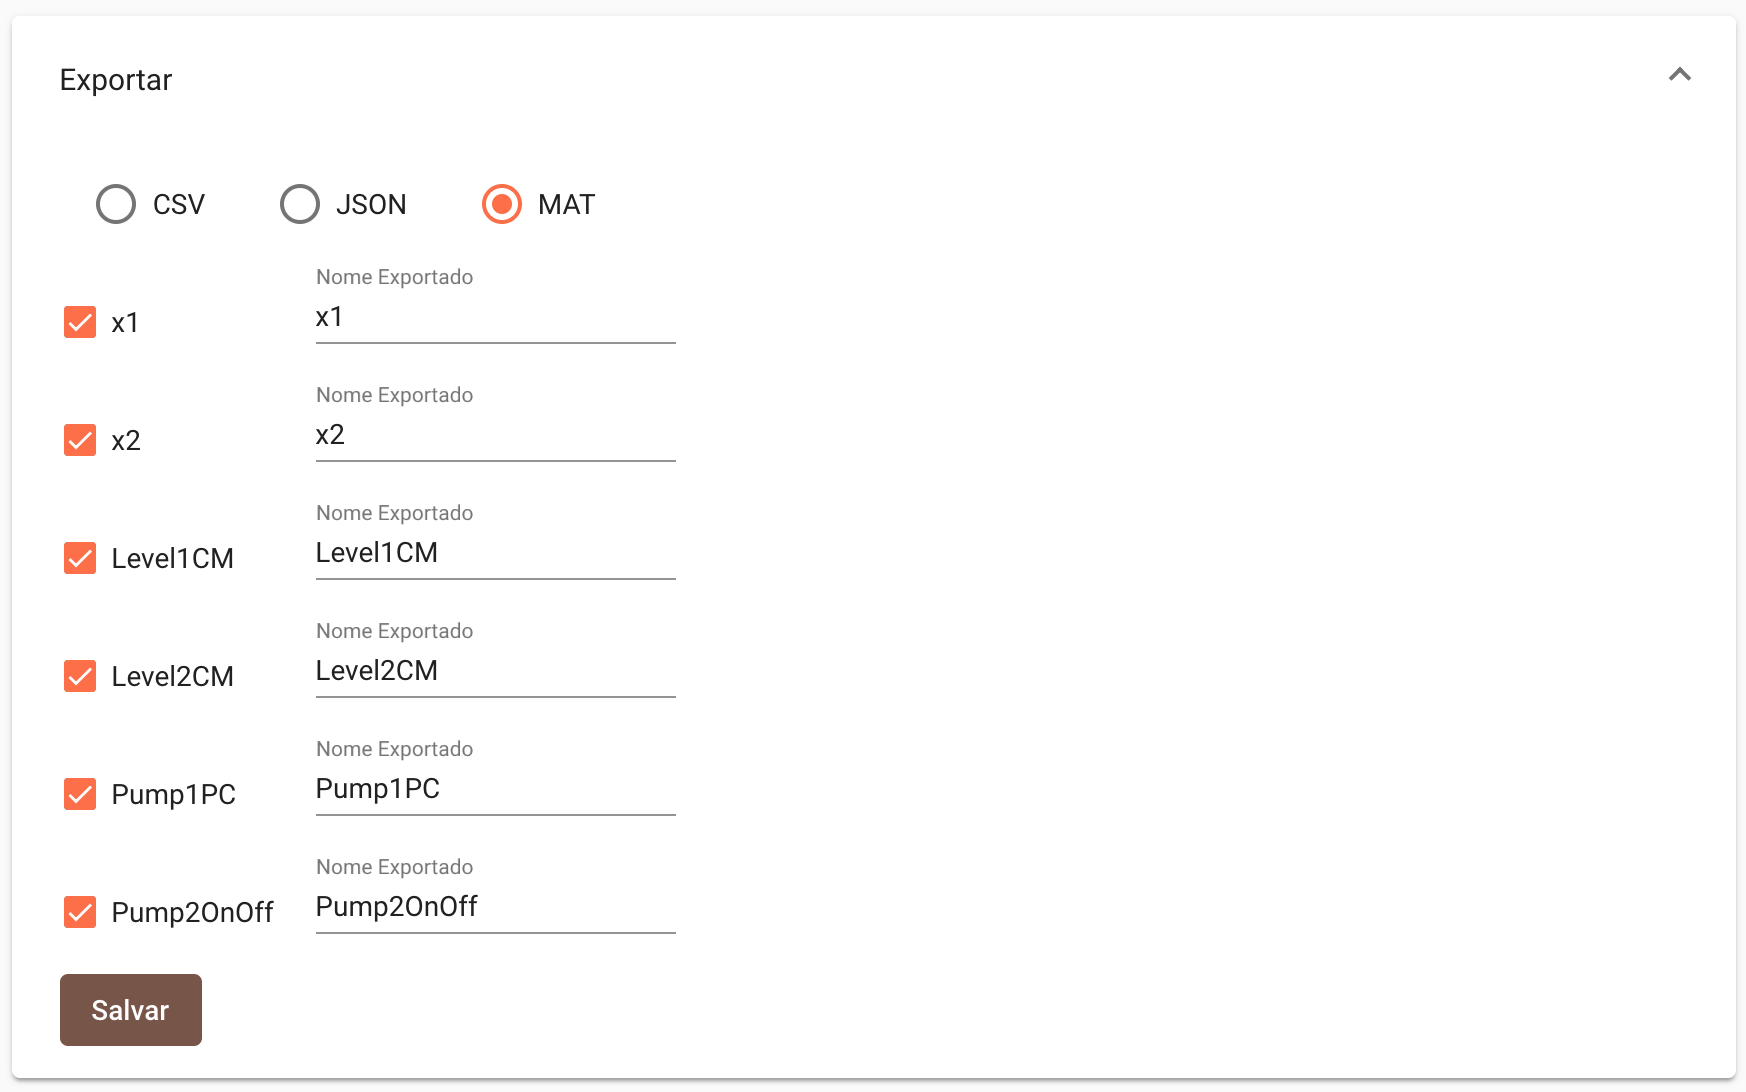
\includegraphics[width=0.9\textwidth]{imgs/graphs2}
    \caption[Exportar dados]{Exportar dados}%
    \label{fig:graphs2}
\end{figure}

Logo em seguida têm-se uma lista de variáveis com \textit{checkboxes} e caixas
de texto. As variáveis com o \textit{checkbox} selecionado serão exportadas, e o
nome definido na caixa de texto será utilizado no arquivo final, ao invés do
nome da variável, permitindo assim que as variáveis sejam renomeadas durante a
exportação. Ao clicar em \textit{Salvar} um arquivo no formato especificado é
gerado e uma janela de salvar arquivo é exibida, permitindo escolher o local
onde o arquivo será salvo.

A seção \textit{Gráficos}, mostradas na Figura~\ref{fig:graphs3}, permite
adicionar gráficos contendo as curvas de uma ou mais variáveis. As variáveis
disponíveis serão as entradas, saídas e aquelas definidas no dicionário
\textit{log}.

\begin{figure}[ht!]
    \centering
    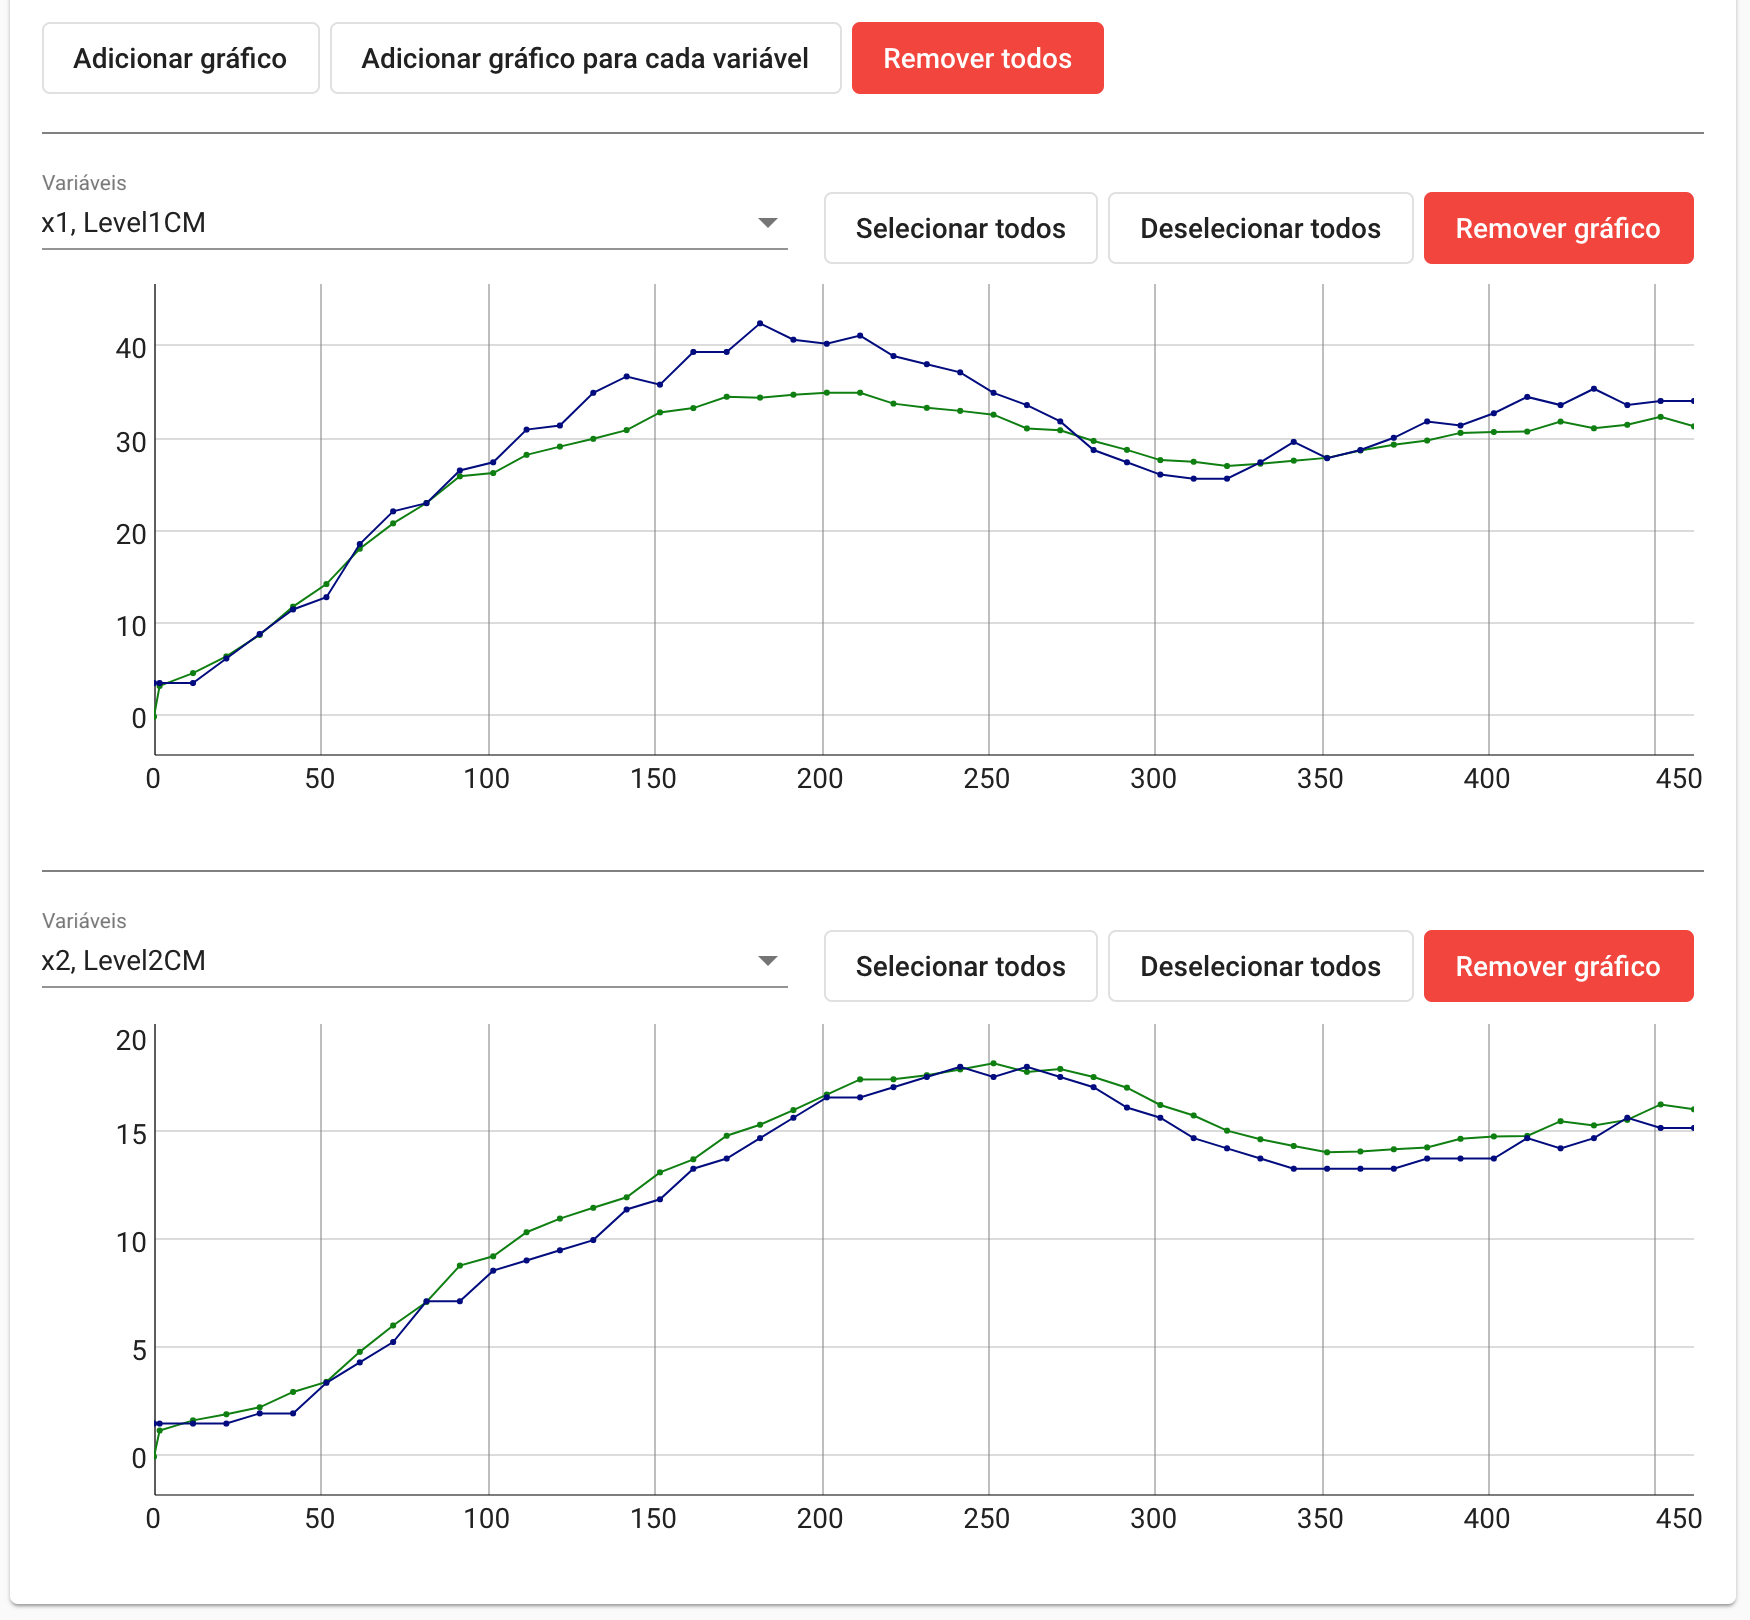
\includegraphics[width=0.9\textwidth]{imgs/graphs3}
    \caption[Gráficos]{Gráficos}%
    \label{fig:graphs3}
\end{figure}

É possível adicionar e remover gráficos sem restrição. Para cada gráfico pode-se
selecionar quais variáveis serão exibidas nele. Algumas funcionalidades de
conveniência estão disponíveis, como a opção de adicionar um gráfico para cada
variável e de selecionar ou deselecionar todas as variáveis em um único gráfico.

Ao passar o \textit{mouse} sobre o gráfico, a legenda é exibida mostrando o nome
de cada curva na mesma cor da linha utilizada no gráfico, além do valor no ponto
atual. O valor eixo \(x\), que sempre representa o tempo em segundos, é exibido
antes de todas as variáveis.

\begin{figure}[ht!]
    \centering
    
\includegraphics[width=0.9\textwidth]{imgs/graphs4}
    \caption[Teste em execução]{Teste em execução}%
    \label{fig:graphs4}
\end{figure}

Quando um teste está em execução, ele é marcado com o símbolo
\img{imgs/running}, como pode ser visto na Figura~\ref{fig:graphs4}. O botão
\textit{Remover} (\img{imgs/remove}) é substituído pelo botão \textit{Parar}
(\img{imgs/stop}). Os gráficos de um teste em execução são atualizados a cada
segundo. Essa atualização requer considerável processamento pelo aplicativo
\textbf{moirai}, sendo recomendado não manter o módulo \textit{Gráficos} aberto
durante a execução de um teste em um computador com baixo poder de
processamento. A lista de gráficos disponíveis também é atualizada a cada
segundo, fazendo com que um teste em execução não seja listado imediatamente,
mas após alguns segundos.
